\setlength{\columnsep}{3pt}
\begin{flushleft}
	
	\begin{itemize}
		\item A hard disk can be divided into several partitions. 
		\item Before understanding types of partitions, let's first see:
		\paragraph{What is MBR?}
			\item The first \textbf{512 bytes} of HDD consists of \textbf{master boot recorder (MBR)} that consists of:
			\begin{itemize}
				\item Bootloader (446 bytes in size) - Will learn more on this in later chapter.
				\item \textbf{Partition Table} - 16 bytes in size. Can stores entry of maximum 4 partitions (4 byte entry for each partition).
				\item Magic number (2 bytes in size) - Will learn more on this in later chapter.
			\end{itemize}
	
		\begin{figure}[h!]
			\centering
			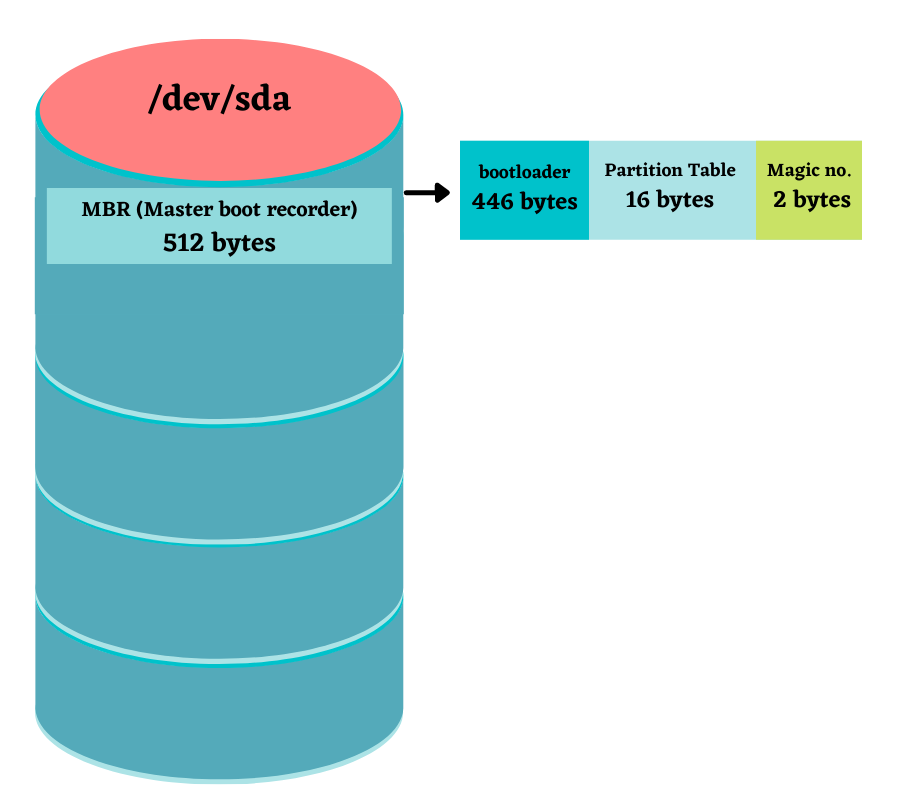
\includegraphics[scale=.5]{content/chapter8/images/mbr.png}
			\caption{MBR}
			\label{mbr_naming}
		\end{figure}		
		
		\newpage
		\item As the partition table in MBR can hold only 4 entries, there can be only \textbf{four partitions in hard disks called primary partitions}.
		\begin{figure}[h!]
			\centering
			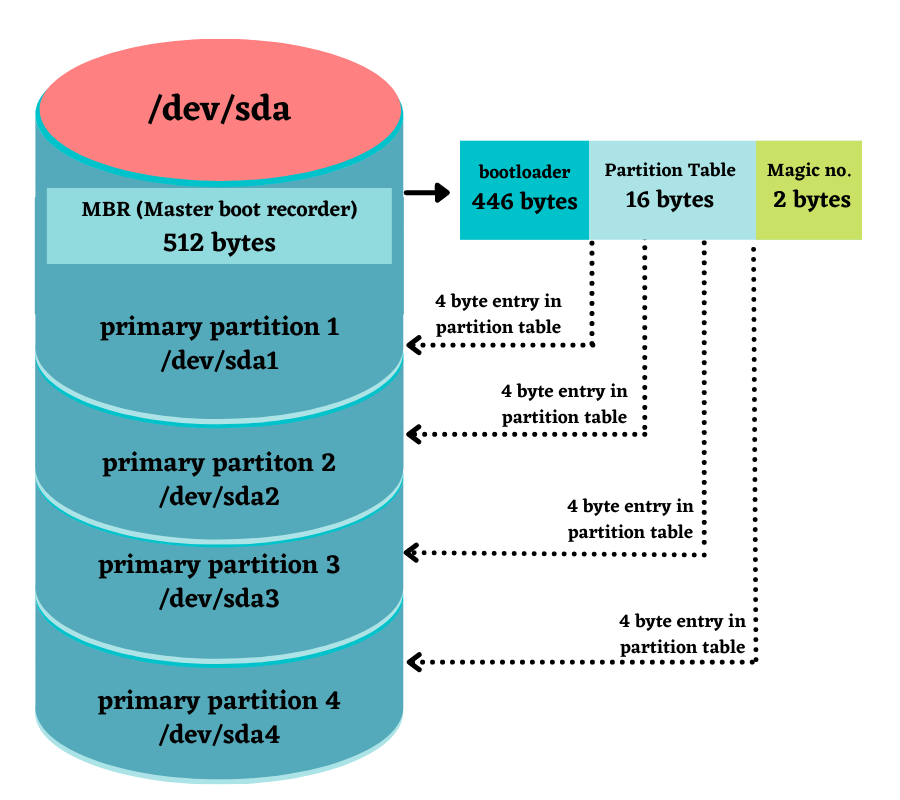
\includegraphics[scale=.5]{content/chapter8/images/primary.png}
			\caption{Primary partitions}
			\label{primary_naming}
		\end{figure}		
		\item Ordering of primary partition is not fixed.
		
	\end{itemize}
	
\end{flushleft}

\newpage

